\subsection{Discharging Circuitry}

The discharging \hyperlink{sch:discharging}{circuitry} provides a means to determine the bulk capacitance value of the \gls{dut} from the RC time constant. Once the \gls{dut} is charged via the operation described in Section: \ref{sec:charging}, the charging relay will open and the high-current discharge relay will close. The transimpedance amplifier described in Section: \ref{sec:iMeas} will measure the current through the \gls{dut} as it decays.

There are 3 switched discharge stages that allow for the decay rate to be regulated. Each stage allows for a range of voltages and capacitances needed to stay within safety and operational constraints. As seen in Figure: \ref{fig:opArea}, there are two constraints on both the voltage and capacitance. The maximum voltage is constrained by either the power rating on the lowest valued resistor or the overall safety limit of $500$VDC. The minimum capacitance value is constrained by setting a $100$ \gls{adc} samples per time constant with a sampling rate of $240$KSPS.

\begin{figure}[ht!]
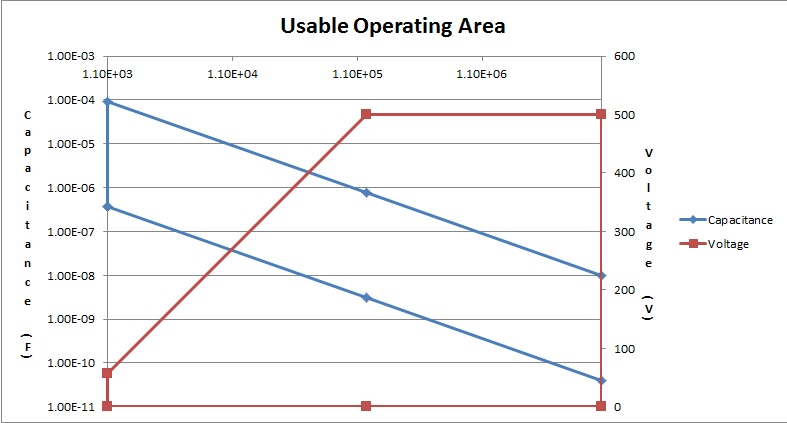
\includegraphics[keepaspectratio=true,width=3in]{./figures/circEx/operatingArea.jpg}
\centering
\caption{Operating Area}
\label{fig:opArea}
\end{figure}


